% =====================================================================
%  Présentation entretien doctorat — Orange Research, 13 mai 2026
%  "La syntaxe espagnole se cache-t-elle dans mBERT ?"
% =====================================================================
\documentclass[aspectratio=169,11pt]{beamer}

\usetheme{default}
\usecolortheme{seagull}
\setbeamertemplate{navigation symbols}{}
\setbeamertemplate{footline}[frame number]
\setbeamertemplate{itemize items}[circle]
\setbeamercolor{frametitle}{fg=black}
\setbeamercolor{title}{fg=black}
\setbeamerfont{frametitle}{size=\large, series=\bfseries}
\setbeamerfont{title}{size=\Large, series=\bfseries}

\usepackage[T1]{fontenc}
\usepackage[utf8]{inputenc}
% French babel not installed in this TeX distribution; we rely on
% inputenc + lmodern for accented characters and use literal Unicode
% guillemets « » directly.
\usepackage{lmodern}
\usepackage{amsmath, amssymb}
\usepackage{booktabs}
\usepackage{tikz}
\usetikzlibrary{positioning, arrows.meta, shapes.geometric, fit, backgrounds}
\usepackage{pgfplots}
\pgfplotsset{compat=1.18}
\usepackage{xcolor}
\usepackage{xspace}

\definecolor{accent}{RGB}{255, 121, 0}
\definecolor{frozenblue}{RGB}{100, 140, 200}
\definecolor{probegreen}{RGB}{80, 160, 80}
\setbeamercolor{structure}{fg=accent}

\newcommand{\mbert}{m\textsc{BERT}\xspace}
\newcommand{\ancora}{UD\_Spanish-AnCora\xspace}

\title{Les \emph{transformers} (type BERT) encodent-ils la syntaxe d'une langue ?}
\author{Marcos Lahoz Yague}
\date{}

\begin{document}

% =====================================================================
% 1. Titre
% =====================================================================
\begin{frame}
  \titlepage
\end{frame}

% =====================================================================
% 2a. Le langage est arborescent
% =====================================================================
\begin{frame}{Le langage est \emph{arborescent}}
  \begin{columns}[T]
    \column{0.5\textwidth}
    \vspace{0.3cm}
    On représente une phrase comme un \alert{arbre de dépendances} :
    \begin{itemize}\setlength\itemsep{6pt}
      \item chaque mot a \alert{exactement un mot-tête} --- le mot
            dont il dépend grammaticalement ;
      \item la seule exception est la \alert{racine}, sans tête,
            typiquement le verbe principal ;
      \item chaque arête porte une étiquette
            (\textit{nsubj}, \textit{obj}, \textit{det}\ldots)
            qui nomme la relation grammaticale.
    \end{itemize}


    \column{0.48\textwidth}
    \centering
    \vspace{0.3cm}
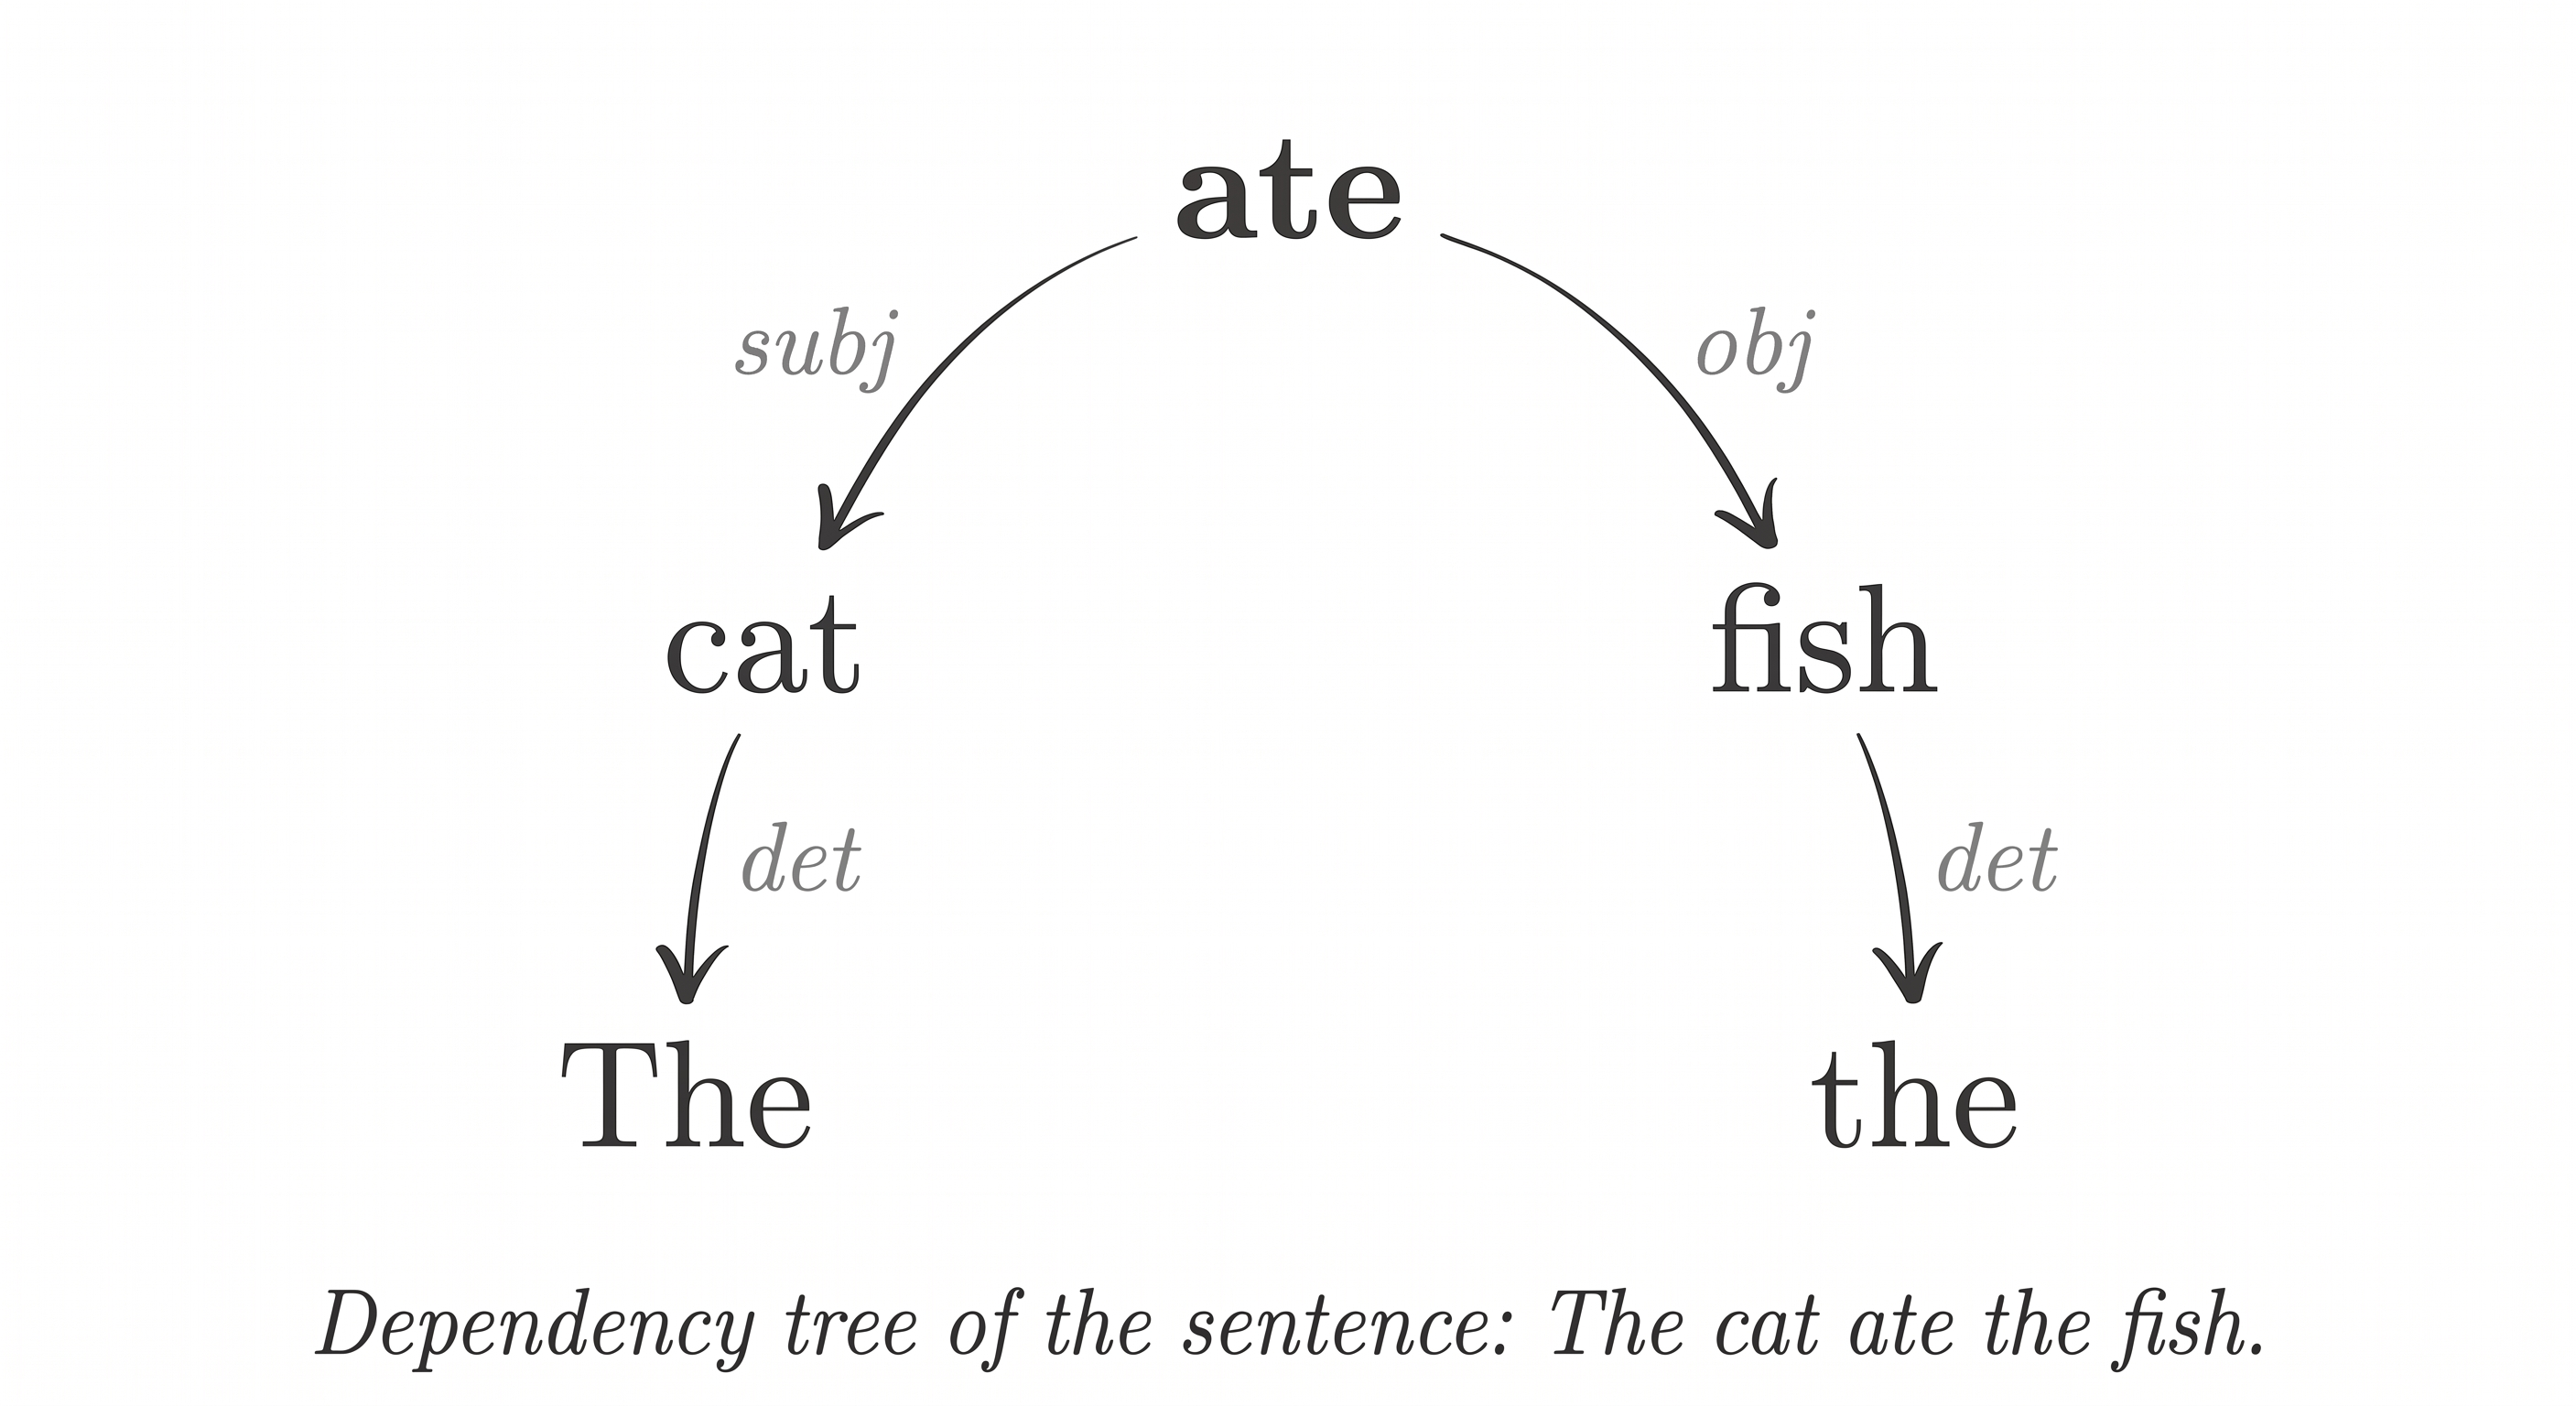
\includegraphics[width=\linewidth]{figures/dependency_tree_v2.png}
  \end{columns}
\end{frame}

% =====================================================================
% 2b. Deux métriques sur l'arbre
% =====================================================================
\begin{frame}{Deux métriques naturelles sur l'arbre}
  \vspace{0.15cm}
  Avec cette définition de la syntaxe (un arbre de dépendances), on
  associe à chaque phrase \alert{deux quantités numériques} naturelles.

  \vspace{0.35cm}
  \begin{columns}[T]

    % ---------- Profondeur ----------
    \column{0.48\textwidth}
    \centering
    \textbf{1. Profondeur d'un mot} \quad $\mathrm{depth}_T(w_i)$\\[2pt]
    {\footnotesize\emph{Nombre d'arêtes du mot jusqu'à la racine.}}

    \vspace{0.25cm}
    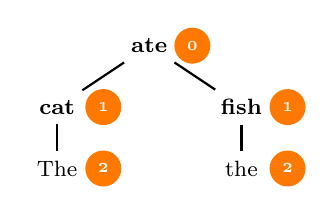
\begin{tikzpicture}[scale=0.78, every node/.style={font=\footnotesize}]
      \node (v) at (0,3) {\textbf{ate}};
      \node (s) at (-1.5,2) {\textbf{cat}};
      \node (a) at (-1.5,1) {The};
      \node (o) at (1.5,2) {\textbf{fish}};
      \node (b) at (1.5,1) {the};
      \draw[thick] (v) -- (s);
      \draw[thick] (v) -- (o);
      \draw[thick] (s) -- (a);
      \draw[thick] (o) -- (b);
      \node[circle, fill=accent, text=white, font=\tiny\bfseries,
            inner sep=0pt, minimum size=13pt, anchor=west] at (0.40, 3)  {0};
      \node[circle, fill=accent, text=white, font=\tiny\bfseries,
            inner sep=0pt, minimum size=13pt, anchor=west] at (-1.05, 2) {1};
      \node[circle, fill=accent, text=white, font=\tiny\bfseries,
            inner sep=0pt, minimum size=13pt, anchor=west] at ( 1.95, 2) {1};
      \node[circle, fill=accent, text=white, font=\tiny\bfseries,
            inner sep=0pt, minimum size=13pt, anchor=west] at (-1.05, 1) {2};
      \node[circle, fill=accent, text=white, font=\tiny\bfseries,
            inner sep=0pt, minimum size=13pt, anchor=west] at ( 1.95, 1) {2};
    \end{tikzpicture}

    \vspace{0.15cm}
    {\footnotesize Position dans la hiérarchie. Le verbe principal est
    toujours à 0.}

    % ---------- Distance ----------
    \column{0.48\textwidth}
    \centering
    \textbf{2. Distance entre deux mots} \quad $d_T(w_i, w_j)$\\[2pt]
    {\footnotesize\emph{Nombre d'arêtes du chemin unique qui les relie.}}

    \vspace{0.25cm}
    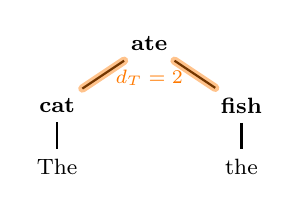
\begin{tikzpicture}[scale=0.78, every node/.style={font=\footnotesize}]
      \node (v) at (0,3) {\textbf{ate}};
      \node (s) at (-1.5,2) {\textbf{cat}};
      \node (a) at (-1.5,1) {The};
      \node (o) at (1.5,2) {\textbf{fish}};
      \node (b) at (1.5,1) {the};
      \draw[thick] (v) -- (s);
      \draw[thick] (v) -- (o);
      \draw[thick] (s) -- (a);
      \draw[thick] (o) -- (b);
      % Highlight path cat -- ate -- fish (distance 2)
      \draw[line width=3pt, accent, opacity=0.45,
            line cap=round] (s) -- (v) -- (o);
      % Distance label
      \node[accent, font=\scriptsize\bfseries] at (0, 2.45) {$d_T = 2$};
    \end{tikzpicture}

    \vspace{0.15cm}
    {\footnotesize $d_T(\text{cat},\text{fish}) = 2$,\;
                   $d_T(\text{The},\text{book}) = 3$,\;
                   $d_T(\text{The},\text{the}) = 4$.}

  \end{columns}

\end{frame}



% =====================================================================
% Lead : la réponse de H&M
% =====================================================================
\begin{frame}{Hewitt \& Manning (NAACL 2019) : ce qu'ils essaient}
  \vspace{0.3cm}
  Ils s'attaquent à \alert{la même question}, dans un cadre concret :
  \begin{itemize}\setlength\itemsep{6pt}
    \item Encodeur : \alert{BERT-base} (12 couches, 768 dim, figé).
    \item Langue : \alert{anglais}.
    \item Treebank : Penn Treebank (Wall Street Journal).
  \end{itemize}

  \vspace{0.6cm}
  \centering
  \large
  \alert{Question opérationnelle :} peut-on retrouver les distances $d_T$
  à partir des vecteurs contextuels ?
\end{frame}

% =====================================================================
% 4. Qu'est-ce qu'une sonde ?
% =====================================================================
\begin{frame}{Probing structurel : setup}
  \begin{columns}[T]
    \column{0.42\textwidth}
    \begin{itemize}\setlength\itemsep{6pt}
      \item Modèle \alert{figé}.
      \item Sonde \alert{linéaire} sur une couche cachée.
    \end{itemize}

    \vspace{0.4cm}
    \[
      \|B(h_i - h_j)\|_2^2 \;=\; \hat d_{ij} \;\approx\; d_T(w_i, w_j)
    \]

    \vspace{0.2cm}
    {\footnotesize Projection linéaire $B$ apprise par régression
    $\ell_1$ sur les distances de l'arbre. Seule supervision :
    les distances $d_T$. La sonde n'accède qu'aux vecteurs.}

    \column{0.55\textwidth}
    \centering
    \vspace{0.1cm}
\hspace*{-2.5cm}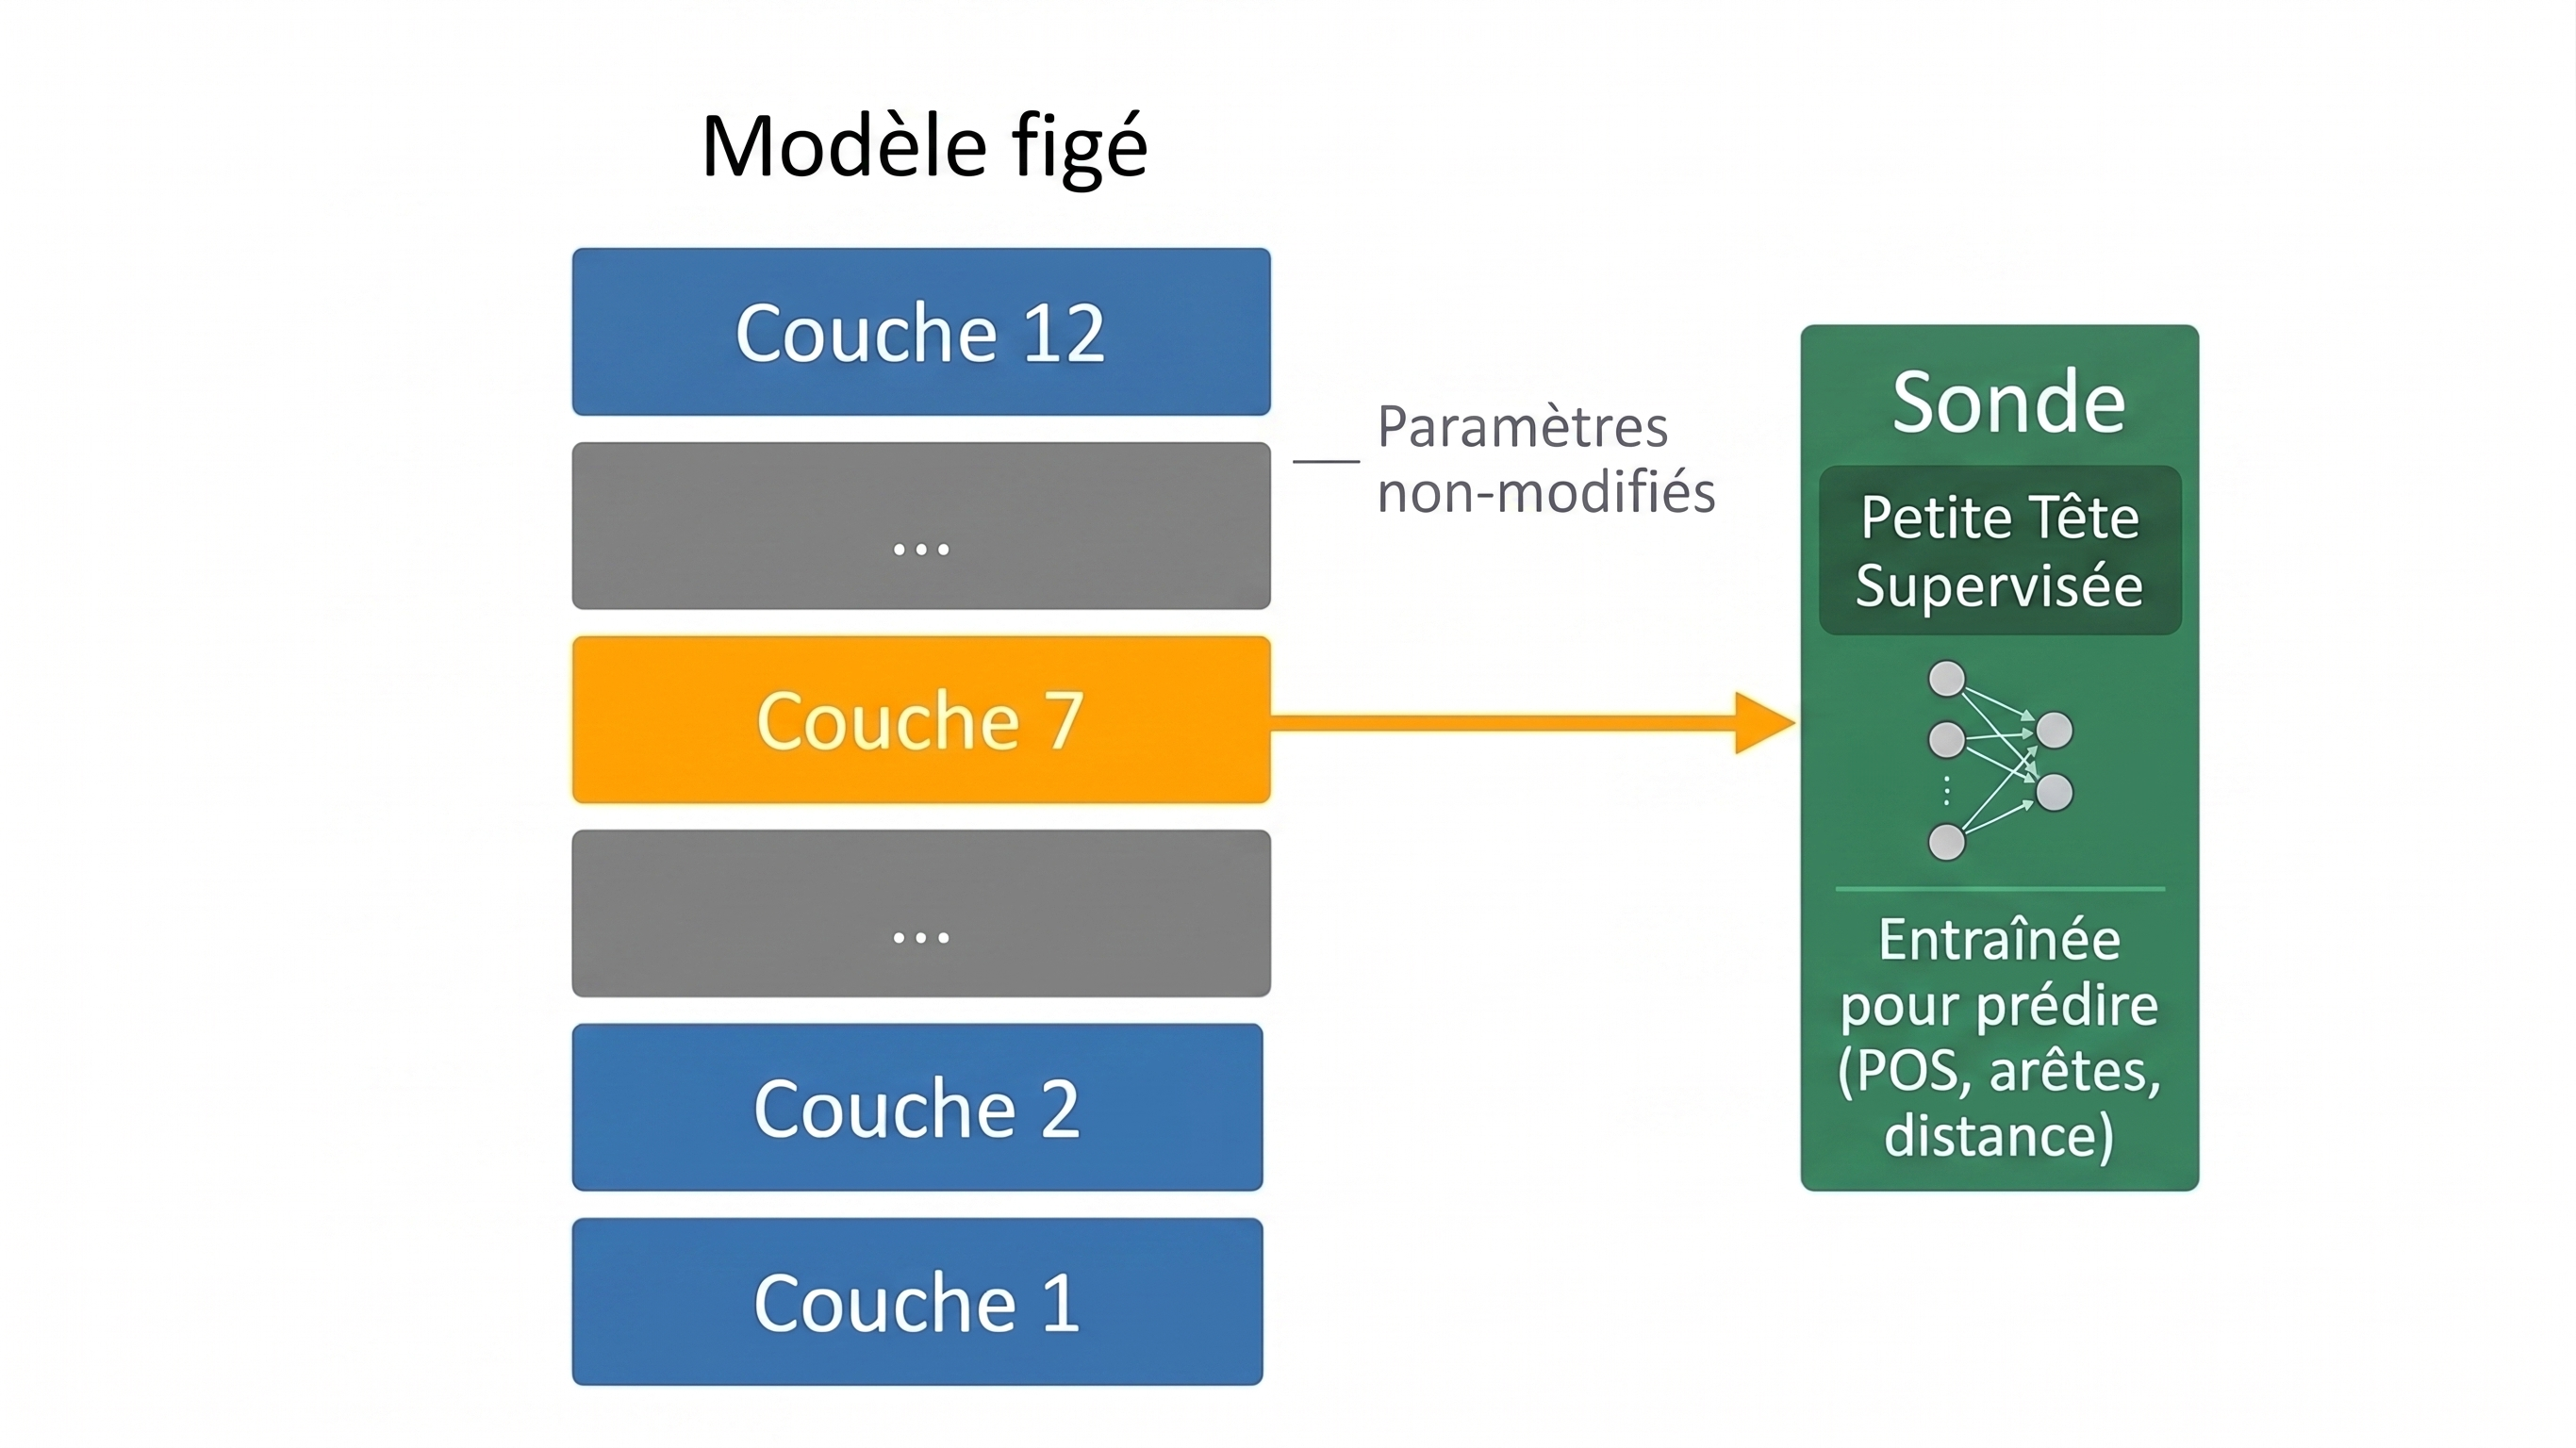
\includegraphics[width=1.30\linewidth]{figures/probe_Schema.png}
  \end{columns}
\end{frame}

% =====================================================================
% Métriques d'évaluation -- Spearman
% =====================================================================
\begin{frame}{\'Evaluer la sonde (1/2) : Spearman $\rho$}
  \begin{columns}[T]

    % ---------- Left: definition + formula ----------
    \column{0.55\textwidth}
    \vspace{0.1cm}
    Pour chaque mot $w_i$, on compare \alert{l'ordre} de deux listes :\\
    $\{\hat d(w_i, w_j)\}$ vs $\{d_T(w_i, w_j)\}$.

    \vspace{0.4cm}
    \[
      \rho_i \;=\; 1 \;-\; \frac{6 \sum_{j \neq i}
        \bigl(\mathrm{pos}_{\hat d}(w_j) - \mathrm{pos}_{d_T}(w_j)\bigr)^2}
                                    {n(n^2-1)}
    \]

    \vspace{0.1cm}
    {\footnotesize $\mathrm{pos}$ : position de $w_j$ dans l'ordre
    croissant des distances vers $w_i$.}

    \vspace{0.3cm}
    {\footnotesize \alert{$\rho = +1$} : ordres identiques. \quad
    $\rho = -1$ : oppos\'es.}

    \vspace{0.3cm}
    {\footnotesize Le coefficient final est une moyenne \alert{$\rho_{5\text{-}50}$}
    sur les $\rho_i$ \emph{(voir backup pour les d\'etails)}.}

    % ---------- Right: example ----------
    \column{0.42\textwidth}
    \centering
    \vspace{0.2cm}
    {\footnotesize Exemple : depuis « ate »}

    \vspace{0.15cm}
    \footnotesize
    \begin{tabular}{@{}lcc@{}}
      \toprule
      $w_j$  & $d_T$ & $\hat d$ \\
      \midrule
      cat    & 1     & 0{,}8     \\
      fish   & 1     & 1{,}2     \\
      The    & 2     & 1{,}9     \\
      the    & 2     & 2{,}1     \\
      \bottomrule
    \end{tabular}

    \vspace{0.3cm}
    {\footnotesize Valeurs diff\'erentes,\\ \alert{m\^eme ordre}
    $\Rightarrow \rho_i = 1$.}
  \end{columns}
\end{frame}

% =====================================================================
% Métriques d'évaluation -- UUAS
% =====================================================================
\begin{frame}{\'Evaluer la sonde (2/2) : UUAS}
  \vspace{0.1cm}
  \centering
  {\footnotesize\emph{Unlabeled Undirected Attachment Score}}

  \vspace{0.4cm}
  \begin{columns}[T]
    \column{0.50\textwidth}
    \textbf{Recette :}
    \begin{itemize}\setlength\itemsep{4pt}
      \item \`A partir de $\hat d$, construire un \alert{arbre couvrant minimum}.
      \item Comparer ses ar\^etes \`a celles de l'arbre vrai.
      \item \textbf{UUAS} = \alert{fraction d'ar\^etes correctement retrouv\'ees}.
    \end{itemize}

    \column{0.45\textwidth}
    \centering
    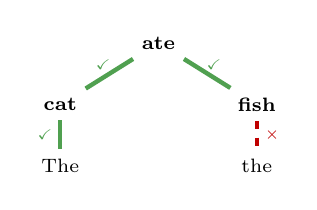
\begin{tikzpicture}[scale=0.78, every node/.style={font=\scriptsize}]
      \node (v) at ( 0, 2.0) {\textbf{ate}};
      \node (c) at (-1.6, 1.0) {\textbf{cat}};
      \node (f) at ( 1.6, 1.0) {\textbf{fish}};
      \node (T) at (-1.6, 0.0) {The};
      \node (t) at ( 1.6, 0.0) {the};
      \draw[ultra thick, probegreen] (v) -- (c);
      \draw[ultra thick, probegreen] (v) -- (f);
      \draw[ultra thick, probegreen] (c) -- (T);
      \draw[ultra thick, red!75!black, dashed] (f) -- (t);
      \node[probegreen, font=\tiny\bfseries] at (-0.9, 1.65) {$\checkmark$};
      \node[probegreen, font=\tiny\bfseries] at ( 0.9, 1.65) {$\checkmark$};
      \node[probegreen, font=\tiny\bfseries] at (-1.85, 0.5) {$\checkmark$};
      \node[red!75!black, font=\tiny\bfseries] at ( 1.85, 0.5) {$\times$};
    \end{tikzpicture}

    \vspace{0.2cm}
    {\footnotesize Ex. : 3 sur 4 = \alert{$0{,}75$}.}
  \end{columns}
\end{frame}

% =====================================================================
% Résultat de H&M sur l'anglais
% =====================================================================
\begin{frame}{Résultat de H\&M sur l'anglais : \alert{OUI}}
  \centering
  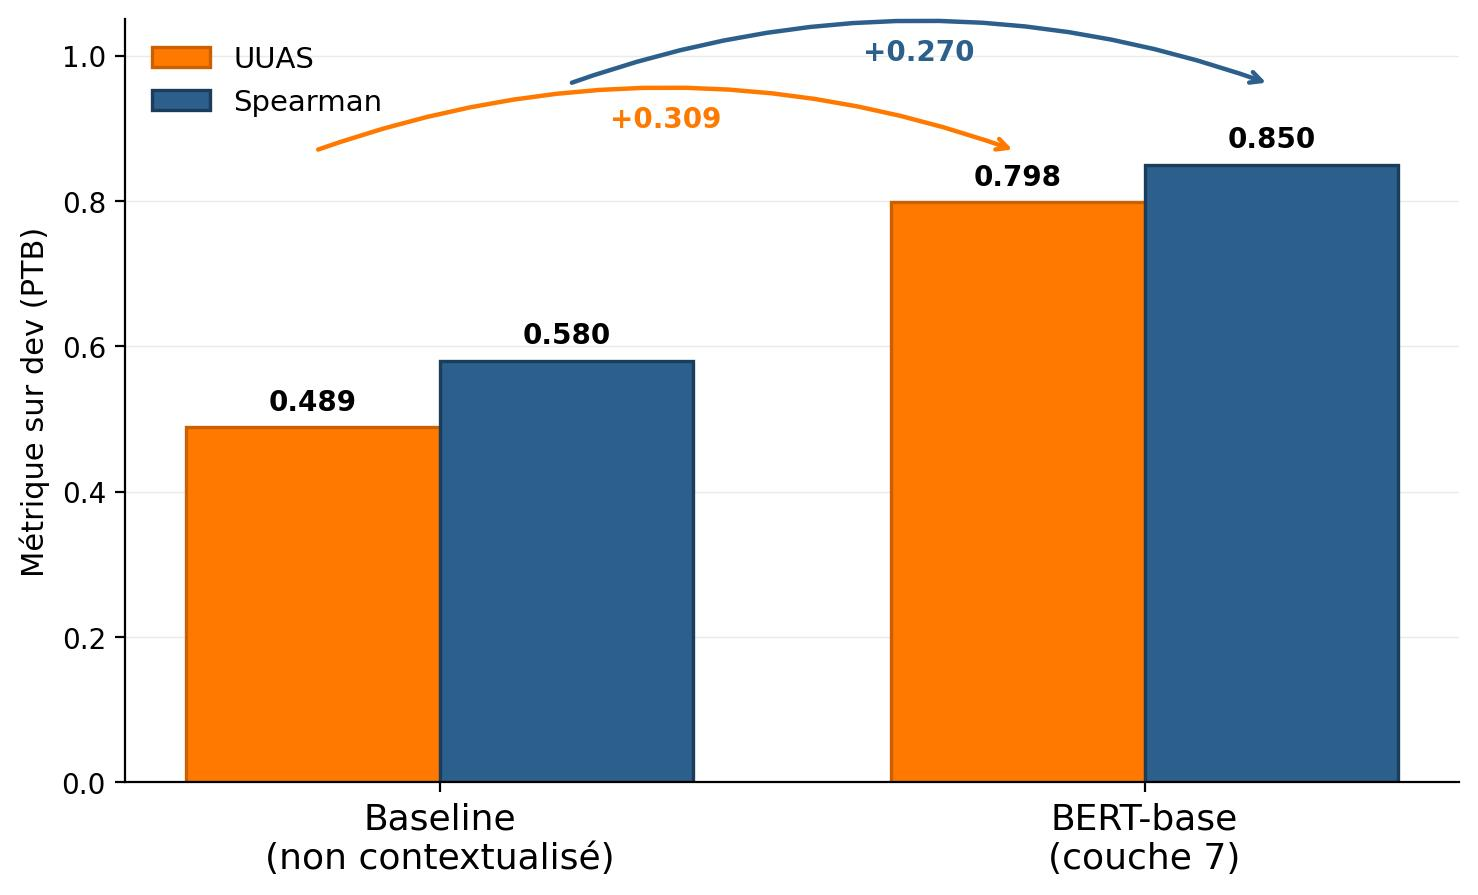
\includegraphics[width=0.78\textwidth]{figures/hm_baseline_vs_bert.jpg}

  \vspace{0.4cm}
  \large
  $\Rightarrow$ la syntaxe \emph{vit} dans la géométrie de BERT.
\end{frame}



% =====================================================================
% 7. Ce que nous ajoutons
% =====================================================================
\begin{frame}{Ce que nous ajoutons}
  Hewitt \& Manning ont répondu à la question sur \alert{BERT anglais}.
  Deux suites naturelles restent ouvertes :

  \vspace{0.4cm}
  \begin{enumerate}\setlength\itemsep{8pt}
    \item \textbf{Transfert cross-lingue.} La même géométrie syntaxique
          existe-t-elle dans \alert{BERT multilingue} pour des langues
          autres que l'anglais ? Concrètement : fonctionne-t-elle sur
          \alert{l'espagnol} via mBERT ?
    \item \textbf{Forme rigide ou directions à amplifier ?} L'arbre
          syntaxique est-il déjà présent comme une \alert{figure
          géométrique rigide} dans l'espace de BERT (la sonde n'a qu'à
          \emph{tourner}), ou est-il codé dans \alert{certaines
          directions} que la sonde doit \emph{étirer} pour le rendre
          lisible ?
  \end{enumerate}

  \vspace{0.5cm}
  Nos deux contributions répondent à ces deux questions :
  \begin{itemize}
    \item Réplication couche par couche sur \ancora.
    \item \textbf{Sonde isométrique} --- une variante contrainte qui
          isole la rotation de l'étirement.
  \end{itemize}
\end{frame}
% =====================================================================
% 12. Résultat 1 : layer sweep
% =====================================================================
\begin{frame}{Résultat 1 --- la syntaxe espagnole pique à la couche 7}
  \centering
  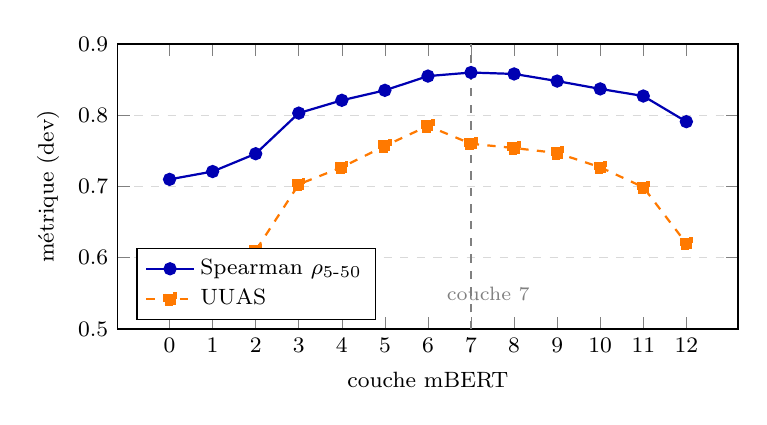
\begin{tikzpicture}
  \begin{axis}[
    width=0.78\textwidth, height=5.2cm,
    xlabel={couche mBERT},
    ylabel={métrique (dev)},
    xtick=data,
    legend pos=south west, legend cell align=left,
    legend style={font=\footnotesize},
    ymin=0.5, ymax=0.9, ymajorgrids,
    grid style={dashed, gray!30},
    label style={font=\footnotesize},
    tick label style={font=\footnotesize},
  ]
  \addplot[mark=*, thick, color=blue!70!black] coordinates {
    (0,0.710) (1,0.721) (2,0.746) (3,0.803) (4,0.821) (5,0.835)
    (6,0.855) (7,0.860) (8,0.858) (9,0.848) (10,0.837) (11,0.827) (12,0.791)
  };
  \addlegendentry{Spearman $\rho_{5\text{-}50}$}
  \addplot[mark=square*, dashed, thick, color=accent] coordinates {
    (0,0.562) (1,0.562) (2,0.610) (3,0.703) (4,0.727) (5,0.757)
    (6,0.785) (7,0.760) (8,0.754) (9,0.747) (10,0.727) (11,0.699) (12,0.620)
  };
  \addlegendentry{UUAS}
  \draw[gray, dashed] (axis cs:7,0.5) -- (axis cs:7,0.9);
  \node[gray, font=\scriptsize] at (axis cs:7.4,0.55) {couche 7};
  \end{axis}
  \end{tikzpicture}

  \footnotesize
  \begin{itemize}\setlength\itemsep{2pt}
    \item Courbe en cloche reproduisant celle de Hewitt-Manning sur l'anglais.
    \item Meilleure couche 7 : \alert{Spearman $0{,}860$},
          \alert{UUAS $0{,}760$}.
  \end{itemize}
\end{frame}

% =====================================================================
% 13. Comparaison anglais vs espagnol
% =====================================================================
\begin{frame}{Transfert cross-lingue : seulement $-4$ points d'UUAS}
  \centering
  \vspace{0.3cm}
  \begin{tabular}{lcc}
    \toprule
                         & \textbf{H\&M (BERT anglais, PTB)} & \textbf{Nous (mBERT, AnCora)} \\
    \midrule
    Meilleure couche     & 7--8              & \textbf{7} \\
    Spearman distance    & $0{,}850$         & \textbf{0{,}860} \\
    UUAS                 & $0{,}798$         & \textbf{0{,}760} \\
    Rang de la sonde     & 128               & 128 \\
    \bottomrule
  \end{tabular}

  \vspace{0.5cm}
  \begin{itemize}\setlength\itemsep{4pt}
    \item Même organisation en cloche sur les couches, pic décalé d'au
          plus une couche.
    \item Spearman \emph{légèrement plus haut} en espagnol ; UUAS
          seulement $4$ points en dessous, malgré la dilution
          multilingue de mBERT sur 104 langues.
    \item Forte évidence pour le \alert{sous-espace syntaxique
          indépendant de la langue} (Chi et al., ACL 2020).
  \end{itemize}
\end{frame}

% =====================================================================


% =====================================================================
% 8. La sonde isométrique
% =====================================================================
\begin{frame}{Contribution : la sonde \emph{isométrique}}
  La sonde linéaire \alert{tourne et étire} l'espace mBERT.
  Deux opérations entremêlées. \quad \textbf{Question :} laquelle compte ?

  \vspace{0.5cm}
  \textbf{Sonde isométrique :} contraindre la projection à être orthogonale.
  \[
    B_\mathrm{iso} B_\mathrm{iso}^\top \;=\; I_r
    \qquad \Longrightarrow \qquad
    \kappa(B_\mathrm{iso}) = 1, \;\; \text{rotation seule}
  \]

  \vspace{0.4cm}
  \footnotesize
  \alert{$\kappa(B)$} = \emph{nombre de condition} : rapport entre la plus
  grande et la plus petite valeur singulière de $B$. \\[2pt]
  $\kappa = 1$ : rotation pure, aucun étirement. \quad
  $\kappa \gg 1$ : la sonde \emph{étire} fortement certaines directions
  par rapport aux autres.
\end{frame}

% =====================================================================
% 9. Deux scénarios
% =====================================================================
\begin{frame}{Deux scénarios --- ce que l'expérience peut distinguer}
  \begin{columns}[T]
    \column{0.48\textwidth}
    \centering
    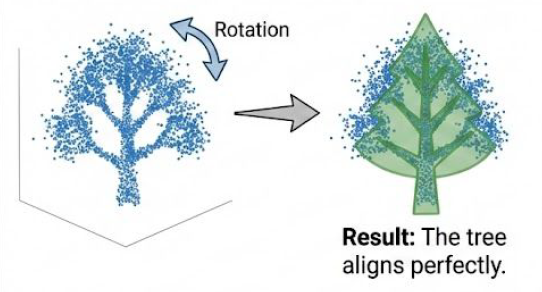
\includegraphics[width=\linewidth]{figures/arbol1.png}

    \vspace{0.3cm}
    \footnotesize
    Si la syntaxe est une \alert{forme rigide} dans l'espace mBERT
    $\;\to\;$ l'isométrique doit \alert{égaler} la sonde linéaire.

    \column{0.48\textwidth}
    \centering
    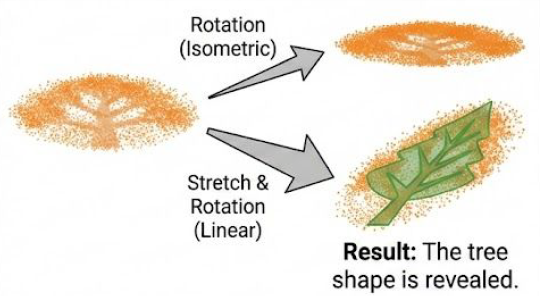
\includegraphics[width=\linewidth]{figures/arbol2.png}

    \vspace{0.3cm}
    \footnotesize
    Si la syntaxe nécessite un \alert{étirement anisotrope}
    $\;\to\;$ l'isométrique \alert{s'effondre}.
  \end{columns}
\end{frame}


% =====================================================================
% 14. Résultat 2 : Pancake Effect
% =====================================================================
\begin{frame}{Résultat 2 --- la syntaxe espagnole \emph{n'est pas} une forme rigide}
  \begin{columns}[T]
    \column{0.55\textwidth}
    \footnotesize
    \begin{tabular}{lrrr}
      \toprule
      Sonde (couche 7) & Spearman & UUAS & $\kappa(B)$ \\
      \midrule
      \textbf{Linéaire} & \textbf{0{,}860} & \textbf{0{,}760} & 3{,}74 \\
      Isométrique       & 0{,}355 & 0{,}272 & 1{,}00 \\
      \midrule
      $\Delta$ relatif & $-59\%$ & $\alert{-64\%}$ & --- \\
      \bottomrule
    \end{tabular}

    \vspace{0.3cm}
    \normalsize
    Contraindre la sonde à être \alert{orthogonale} effondre les
    performances : \alert{$-64\%$} d'UUAS et \alert{$-59\%$} de Spearman.

    \medskip
    \footnotesize
    Spectre singulier de $B$ :
    $\sigma_{\max}{=}0{,}44$, $\sigma_{\min}{=}0{,}12$,
    donc $\kappa = 3{,}74$ (\emph{anisotropie modérée}).

    \column{0.43\textwidth}
    \textbf{Interprétation : l'effet \emph{Pancake}}\\[4pt]
    L'arbre syntaxique espagnol est \alert{aplati} dans des directions
    de faible variance de l'espace mBERT. La sonde doit les
    \emph{amplifier} ($\sim 4{\times}$) pour faire ressortir la
    structure de l'arbre.

  \end{columns}
\end{frame}

% =====================================================================
% Pont vers le multimodal
% =====================================================================
\begin{frame}{Du \emph{probing} syntaxique au \emph{probing} multimodal}
  \begin{columns}[T]
    \column{0.55\textwidth}
    La sonde + diagnostic géométrique développée ici se généralise
    \alert{directement} aux modèles multimodaux.

    \vspace{0.3cm}
    \textbf{Mêmes questions, autre propriété :}
    \begin{itemize}\setlength\itemsep{4pt}
      \item Où vit chaque modalité (vision, audio, texte) ?
      \item Sont-elles \emph{rigidement} préservées
            ($\kappa$ élevé en isolant chacune) ?
      \item À quelle couche l'interaction se cristallise --- et
            observe-t-on un \emph{effondrement modal} ?
    \end{itemize}

    \vspace{0.3cm}
    \footnotesize
    Connecte avec les phénomènes de \emph{modality collapse} rapportés
    par \textbf{Chaudhuri et al.\ ICML 2025}.

    \column{0.43\textwidth}
    \centering
    \footnotesize
    \textbf{Ce travail \quad $\Longrightarrow$ \quad doctorat}

    \vspace{0.3cm}
    \begin{tabular}{ll}
      \toprule
      Aujourd'hui (syntaxe) & Doctorat (multimodal) \\
      \midrule
      couches mBERT  & couches MLLM \\
      axes syntaxiques & axes par modalité \\
      effet Pancake & modality collapse \\
      $\kappa(B)$    & $\kappa$ modal \\
      arbre UD & raisonnement vidéo-QA \\
      \bottomrule
    \end{tabular}

    \vspace{0.4cm}
    Même méthodologie, dimension supérieure.
  \end{columns}
\end{frame}

% =====================================================================
%  BACKUP SLIDES
% =====================================================================
\begin{frame}[plain]
  \centering
  \vspace*{\fill}
  {\Huge\textbf{\textcolor{accent}{Backup}}}\\[0.6cm]
  {\Large slides supplémentaires --- réponses anticipées}
  \vfill
\end{frame}

% ---------------------------------------------------------------------
\begin{frame}{Backup --- Formule exacte de $\rho_{5\text{-}50}$}
  \textbf{Spearman $\rho_i$ (per-mot) :} pour chaque mot $w_i$,
  corr\'elation de rang entre les distances pr\'edites et les vraies
  vers les autres mots.
  \[
    \rho_i \;=\; 1 \;-\; \frac{6 \sum_{j \neq i}
      \bigl(\mathrm{pos}_{\hat d}(w_j) - \mathrm{pos}_{d_T}(w_j)\bigr)^2}
                                  {n(n^2-1)}
  \]
  $n$ : longueur de la phrase. \quad
  $\mathrm{pos}$ : position de $w_j$ dans l'ordre croissant.

  \medskip
  \textbf{1. Moyenne par longueur $\ell$.} On regroupe \emph{tous}
  les $\rho_i$ des mots des phrases de longueur $\ell$ :
  \[
    \bar\rho_\ell \;=\; \frac{1}{\ell \cdot |\mathcal{S}_\ell|}
    \sum_{s \in \mathcal{S}_\ell} \sum_{w_i \in s} \rho_i,
    \qquad \mathcal{S}_\ell \;=\; \text{phrases de longueur }\ell.
  \]

  \textbf{2. Macro-moyenne sur les longueurs.}
  \[
    \alert{\rho_{5\text{-}50}} \;=\; \frac{1}{|L|} \sum_{\ell \in L} \bar\rho_\ell,
    \qquad L = \{5, 6, \ldots, 50\} \cap \text{longueurs pr\'esentes.}
  \]
  Chaque longueur p\`ese autant, ind\'ependamment du nombre de phrases.
\end{frame}


% ---------------------------------------------------------------------
\begin{frame}{Backup --- Données utilisées par H\&M : Penn Treebank (PTB)}
  \textbf{Penn Treebank} (Marcus et al., 1993) --- le treebank
  historique de référence en anglais.
  \begin{itemize}\setlength\itemsep{3pt}
    \item Wall Street Journal, années 1989--1994.
    \item ${\sim}40\,000$ phrases annotées en constituants.
    \item Conversion vers \emph{Stanford Dependencies} (de Marneffe et al., 2006).
    \item Partitions standard : sections 02--21 (train), 22 (dev), 23 (test).
  \end{itemize}

  \vspace{0.4cm}
  \textbf{Pourquoi PTB pour H\&M ?}
  \begin{itemize}\setlength\itemsep{2pt}
    \item Standard de facto pour le parsing en anglais.
    \item Annotations de très haute qualité.
    \item Permet la comparaison directe avec les analyseurs syntaxiques entraînés.
  \end{itemize}

  \vspace{0.3cm}
  \footnotesize
  H\&M testent aussi sur \emph{English Web Treebank} (UD anglais) ---
  résultats similaires.
\end{frame}

% ---------------------------------------------------------------------
\begin{frame}{Backup --- Données : UD\_Spanish-AnCora}
  \begin{columns}[T]
    \column{0.55\textwidth}
    \textbf{Treebank.} Partie espagnole d'AnCora
    (Taulé et al.\ 2008), distribuée via Universal Dependencies
    (\textsc{cc by} 4.0). Texte journalistique, annotations en
    dépendances.

    \vspace{0.4cm}
    \begin{tabular}{lrr}
      \toprule
      partition & phrases & lignes \\
      \midrule
      train & 14\,287 & 453\,039 \\
      dev   &  1\,654 &  53\,476 \\
      test  &  1\,721 &  53\,622 \\
      \bottomrule
    \end{tabular}

    \column{0.43\textwidth}
    \footnotesize
    \textbf{Encodeur.} \texttt{bert-base-multilingual-cased} (mBERT) ---
    104 langues, figé. 12 couches transformer + couche d'entrée.

    \medskip
    \textbf{Sonde.} Rang $r{=}128$, perte $\ell_1$, Adam, 30 époques,
    early stopping (patience 4). Une seule graine.

  \end{columns}
\end{frame}


% ---------------------------------------------------------------------
\begin{frame}{Backup --- L'architecture \emph{transformer} (Vaswani et al., 2017)}
  \begin{columns}[T]
    \column{0.55\textwidth}
    \textbf{Idée centrale :} \emph{self-attention}.

    \medskip
    Pour chaque token $i$ :
    \[
      h_i = \sum_{j} \alpha_{ij}\, V x_j, \quad
      \alpha_{ij} = \mathrm{softmax}_j\!\left(\tfrac{(Q x_i)^\top (K x_j)}{\sqrt{d}}\right)
    \]
    $Q, K, V$ : matrices apprises (\emph{query, key, value}).

    \medskip
    \textbf{Bloc transformer :}
    \begin{itemize}\setlength\itemsep{2pt}
      \item Multi-head self-attention
      \item Feed-forward (MLP par token)
      \item Résidu + LayerNorm
    \end{itemize}
    Empilé $N$ fois.

    \column{0.40\textwidth}
    \centering
    \textbf{Encoder-only}\\[4pt]
    (BERT)\\[10pt]
    \footnotesize
    12 blocs identiques.\\[3pt]
    Chaque token \emph{voit tous les autres} dans les deux directions.\\[3pt]
    Sortie : $h_i \in \mathbb{R}^{768}$ par token.
  \end{columns}
\end{frame}

% ---------------------------------------------------------------------
\begin{frame}{Backup --- BERT en détail}
  \begin{columns}[T]
    \column{0.5\textwidth}
    \textbf{Architecture}
    \begin{itemize}\setlength\itemsep{2pt}
      \item Encoder-only transformer
      \item BERT-base : 12 couches, 768 dim, 110\,M paramètres
      \item BERT-large : 24 couches, 1024 dim, 340\,M paramètres
    \end{itemize}

    \vspace{0.3cm}
    \textbf{Pré-entraînement}
    \begin{itemize}\setlength\itemsep{2pt}
      \item \emph{Masked Language Modeling} : 15\,\% des tokens masqués
      \item \emph{Next Sentence Prediction}
      \item 3{,}3 milliards de mots (Wikipedia EN + BookCorpus)
    \end{itemize}

    \column{0.45\textwidth}
    \textbf{Tokenisation :} WordPiece (sous-mots).\\
    Ex : \texttt{playing} $\to$ \texttt{play, \#\#ing}.

    \vspace{0.3cm}
    \textbf{Tokens spéciaux}
    \begin{itemize}\setlength\itemsep{1pt}
      \item \texttt{[CLS]} : début, classification
      \item \texttt{[SEP]} : séparateur
      \item \texttt{[MASK]} : à prédire
    \end{itemize}

    \vspace{0.3cm}
    \textbf{Sortie :} $h_i \in \mathbb{R}^{768}$ par token, contextuelle.
  \end{columns}
\end{frame}

% ---------------------------------------------------------------------
\begin{frame}{Backup --- mBERT (\texttt{bert-base-multilingual-cased})}
  \textbf{Différences avec BERT :}
  \begin{itemize}\setlength\itemsep{4pt}
    \item Vocabulaire WordPiece partagé sur \alert{104 langues} ($\sim 120$k tokens)
    \item Données : Wikipedia de 104 langues
    \item Échantillonnage exponentiellement lissé (boost des langues à faible ressource)
    \item \alert{Aucune supervision cross-lingue explicite} (pas de paires alignées)
    \item Architecture identique à BERT-base : 12 couches, 768 dim
  \end{itemize}

  \vspace{0.5cm}
  \textbf{Résultat surprenant.} mBERT développe un \alert{sous-espace
  syntaxique partagé} entre les langues, sans qu'on le lui ait
  demandé (Pires et al.\ 2019, Chi et al.\ 2020, ce travail).

  \vspace{0.3cm}
  \emph{Hypothèse :} la contrainte de capacité partagée force le
  modèle à factoriser ce qui est universel.
\end{frame}

% ---------------------------------------------------------------------
\begin{frame}{Backup --- Pourquoi la sonde de \emph{distance} et pas de profondeur ?}
  \textbf{H\&M proposent deux sondes :}
  \[
    \|B(h_i - h_j)\|_2^2 \approx d_T(w_i, w_j) \qquad \text{(distance)}
  \]
  \[
    \|B h_i\|_2^2 \approx \mathrm{depth}_T(w_i) \qquad \text{(profondeur)}
  \]

  \textbf{Pourquoi nous concentrer sur la distance :}
  \begin{enumerate}\setlength\itemsep{4pt}
    \item \textbf{Plus de signal :} $O(n^2)$ paires par phrase contre
          $O(n)$ profondeurs --- même quantité de données, plus de
          supervision.
    \item \textbf{Sens géométrique :} la sonde isométrique pose une
          question sur la \emph{métrique} (préservation des distances).
          La profondeur est une norme depuis l'origine, pas une métrique.
    \item \textbf{Métrique standard} de la littérature dérivée
          (Chi 2020, Reif 2019, Limisiewicz 2020).
  \end{enumerate}

  \vspace{0.3cm}
  \footnotesize
  Notre code (\texttt{ParseDepthTask}) supporte la profondeur ---
  étude complémentaire à faire.
\end{frame}

% ---------------------------------------------------------------------
\begin{frame}{Backup --- Pourquoi la couche 7 (et pas la 6) ?}
  \centering
  \begin{tabular}{lcc}
    \toprule
    Couche & Spearman & UUAS \\
    \midrule
    6           & 0{,}855          & \textbf{0{,}785} \\
    \textbf{7}  & \textbf{0{,}860} & 0{,}760 \\
    \bottomrule
  \end{tabular}

  \vspace{0.5cm}
  \begin{itemize}\setlength\itemsep{3pt}
    \item Sélection de couche par \alert{Spearman} --- protocole H\&M.
    \item Spearman = corrélation directe avec l'objectif d'entraînement
          ($\ell_1$ sur les distances).
    \item UUAS = métrique \emph{dérivée} (construction d'un MST, perte
          de l'information continue).
    \item Sélectionner par UUAS = optimiser une métrique secondaire $\Rightarrow$ \emph{p-hacking}.
    \item Avec une seule graine, le pic UUAS est plus bruité ;
          Spearman est plus stable.
  \end{itemize}
\end{frame}

% ---------------------------------------------------------------------
\begin{frame}{Backup --- Pourquoi un rang $r = 128$ ?}
  \textbf{Choix :} $r = 128 \ll d = 768$.

  \medskip
  \textbf{Comparaison avec H\&M :}
  \begin{itemize}\setlength\itemsep{2pt}
    \item H\&M balayent $r$ jusqu'à $1024$ mais montrent que la
          performance \alert{sature autour de $r = 64$--$128$} pour BERT-base.
    \item Notre $r = 128$ reproduit ce choix optimal.
  \end{itemize}

  \medskip
  \textbf{Justification :}
  \begin{itemize}\setlength\itemsep{2pt}
    \item Reste une vraie projection à basse dimension, pas un autoencodeur.
    \item Réduit le risque de sur-paramétrisation (la sonde apprenant elle-même).
    \item Cohérent avec le principe de \emph{petit modèle}.
  \end{itemize}

  \medskip
  \textbf{À refaire :} sweep de rang ($r \in \{8, 32, 64, 128, 256, 512\}$)
  avec multi-seed pour vérifier que le choix n'est pas critique.
\end{frame}

% ---------------------------------------------------------------------
\begin{frame}{Backup --- La tâche de contrôle (Hewitt \& Liang, EMNLP 2019)}
  \textbf{Question :} la sonde apprend-elle à partir de la
  représentation, ou pourrait-elle apprendre toute structure aléatoire ?

  \medskip
  \textbf{Méthode :}
  \begin{enumerate}\setlength\itemsep{2pt}
    \item Pour chaque \emph{type} de mot, fixer une étiquette aléatoire (consistante).
    \item Entraîner la même sonde sur ces étiquettes aléatoires.
    \item Mesurer la \alert{sélectivité} = perf(vraie tâche) $-$ perf(contrôle).
  \end{enumerate}

  \medskip
  \textbf{Interprétation :}
  \begin{itemize}\setlength\itemsep{2pt}
    \item Sélectivité haute : la sonde exploite vraiment la structure linguistique.
    \item Sélectivité basse : la sonde est trop puissante.
  \end{itemize}

  \medskip
  \textbf{Notre cas :} pas encore fait. Limite reconnue dans les
  slides « Limitations ».
\end{frame}

% ---------------------------------------------------------------------
\begin{frame}{Backup --- Alternatives à mBERT pour l'espagnol}
  \textbf{Encodeurs espagnols monolingues :}
  \begin{itemize}\setlength\itemsep{3pt}
    \item \textbf{BETO} (Cañete et al., 2020) : BERT-base entraîné sur
          \emph{Spanish Unannotated Corpora} ($\sim 3$ milliards de mots).
    \item \textbf{RoBERTa-bne} (BSC, 2022) : RoBERTa-large sur 570\,Go
          de texte espagnol (Biblioteca Nacional de España).
    \item \textbf{MarIA} (BSC, 2022) : famille de modèles GPT-2 et RoBERTa.
  \end{itemize}

  \vspace{0.4cm}
  \textbf{Hypothèse à tester :}
  \begin{itemize}\setlength\itemsep{2pt}
    \item Plus de paramètres dédiés à l'espagnol $\Rightarrow$ géométrie
          syntaxique probablement plus nette.
    \item Quantifier le \emph{coût de la dilution multilingue} de mBERT.
  \end{itemize}

  \vspace{0.3cm}
  \textbf{Statut :} pas mesuré --- extension naturelle du travail.
\end{frame}

% ---------------------------------------------------------------------
\begin{frame}{Backup --- Géométrie des arbres dans l'espace euclidien}
  \textbf{Problème :} les arbres ne s'embedent pas isométriquement
  en euclidien standard.

  \medskip
  \textbf{Théorème de Bourgain :} tout espace métrique fini de $n$
  points s'embed dans $\mathbb{R}^d$ avec distortion $O(\log n)$.

  \medskip
  \textbf{Astuce de H\&M :} utiliser la \alert{distance euclidienne au carré}.
  \[
    \|B h_i - B h_j\|_2^2 \approx d_T(w_i, w_j)
  \]
  La distance \emph{au carré} correspond à une forme bilinéaire
  $h^\top M h$ avec $M = B^\top B$ semi-définie positive.

  \medskip
  \textbf{Lien :} les arbres s'embedent naturellement en géométrie
  hyperbolique (Khrulkov, Sala et al.). La sonde euclidienne est
  une approximation efficace.
\end{frame}

% ---------------------------------------------------------------------
\begin{frame}{Backup --- Le coût du préentraînement BERT}
  \textbf{BERT-base (110\,M paramètres) :}
  \begin{itemize}\setlength\itemsep{2pt}
    \item Wikipedia EN + BookCorpus ($\sim 3{,}3$ milliards de mots).
    \item 4 jours sur 4 Cloud TPU (16 chips).
    \item Coût estimé : $\sim 500\,\$$ (preemptible) à $\sim 7\,000\,\$$ (on-demand, Strubell et al.\ 2019).
  \end{itemize}

  \medskip
  \textbf{BERT-large (340\,M paramètres) :} $\sim$\,60\,000\,\$.

  \medskip
  \textbf{mBERT :} Wikipedia de 104 langues, taille totale comparable.
  Mêmes hyperparamètres que BERT-base.

  \vspace{0.4cm}
  \textbf{Notre coût :} 0\,\euro{} en préentraînement (modèles
  réutilisés). Sondes entraînées sur GPU consumer (G4 sur Colab,
  $\sim$\,3\,h pour le sweep complet).
\end{frame}

% ---------------------------------------------------------------------
\begin{frame}{Backup --- Le \emph{modality collapse} dans les MLLMs}
  \textbf{Phénomène :} dans les Multimodal LLMs, l'information
  distinctive de chaque modalité \alert{s'efface} après quelques
  couches d'intégration.

  \medskip
  \textbf{Référence récente :}
  \begin{itemize}\setlength\itemsep{2pt}
    \item Chaudhuri, Dutta, Bui \& Georgescu, ICML 2025 ---
          \emph{A Closer Look at Multimodal Representation Collapse}.
  \end{itemize}

  \vspace{0.4cm}
  \textbf{Analogie avec l'effet Pancake :}
  \begin{itemize}\setlength\itemsep{2pt}
    \item Syntaxe : la structure d'arbre vit dans une direction
          \emph{aplatie} de l'espace mBERT.
    \item Multimodal : chaque modalité vit dans une direction qui
          s'aplatit progressivement, jusqu'à devenir indistinguable.
  \end{itemize}

  \vspace{0.3cm}
  \alert{Hypothèse :} la sonde isométrique + diagnostic $\kappa$
  pourrait \emph{quantifier} le collapse couche par couche.
\end{frame}

% ---------------------------------------------------------------------
\begin{frame}{Backup --- Comment opérationnaliser « modalité » pour probing ?}
  \textbf{Quatre définitions possibles :}
  \begin{enumerate}\setlength\itemsep{4pt}
    \item \textbf{Signal d'entrée} (pixels, ondes, tokens) --- trivial,
          observable mais peu informatif.
    \item \textbf{Encodeur dédié} (vision, audio) --- structurel mais
          ignore l'intégration.
    \item \alert{\textbf{Sous-espace dans les représentations}} après
          cross-attention --- où le \emph{probing} entre.
    \item \textbf{Capacité comportementale} (réussir une tâche
          modal-spécifique) --- outcome-driven, indirect.
  \end{enumerate}

  \vspace{0.3cm}
  \textbf{Probing visera surtout (3) :} isoler le sous-espace dédié
  à chaque modalité dans les couches d'un MLLM.

  \vspace{0.3cm}
  \textbf{Méthodologie identique à ce travail :}
  \begin{itemize}\setlength\itemsep{2pt}
    \item Sonde linéaire prédisant la présence/contenu d'une modalité.
    \item Sonde isométrique pour tester la rigidité du sous-espace.
    \item $\kappa(B)$ comme diagnostic d'aplatissement.
  \end{itemize}
\end{frame}

\end{document}
